\documentclass[border=6pt]{standalone}
\usepackage{tikz}
\usetikzlibrary{arrows.meta,calc}
\begin{document}
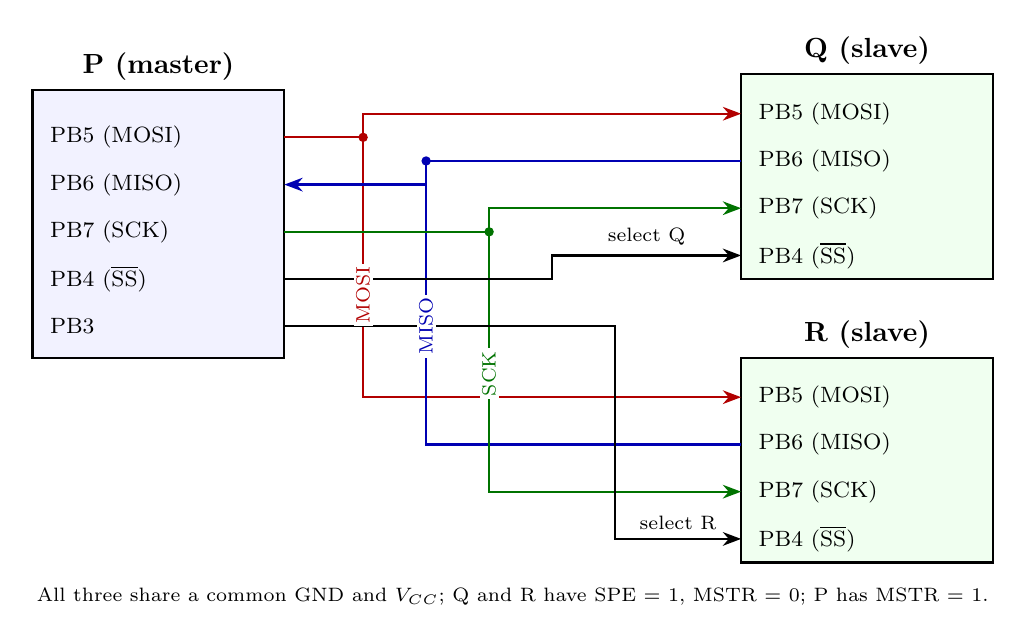
\begin{tikzpicture}[>=Stealth,font=\small,
 chip/.style={draw,thick,fill=blue!5,minimum width=3.0cm,anchor=north west},
 pin/.style={font=\footnotesize,anchor=west},
 dot/.style={circle,fill,inner sep=1.2pt}]
% Master P
\draw[thick,fill=blue!5] (0,0) rectangle (3.2,-3.4);
\node[font=\bfseries] at (1.6,0.3) {P (master)};
\foreach \y/\t in {-0.6/PB5 (MOSI),-1.2/PB6 (MISO),-1.8/PB7 (SCK),-2.4/PB4 ($\overline{\mathrm{SS}}$),-3.0/PB3} \node[pin] at (0.1,\y) {\t};
% Slave Q
\draw[thick,fill=green!6] (9,0.2) rectangle (12.2,-2.4);
\node[font=\bfseries] at (10.6,0.5) {Q (slave)};
\foreach \y/\t in {-0.3/PB5 (MOSI),-0.9/PB6 (MISO),-1.5/PB7 (SCK),-2.1/PB4 ($\overline{\mathrm{SS}}$)} \node[pin] at (9.1,\y) {\t};
% Slave R
\draw[thick,fill=green!6] (9,-3.4) rectangle (12.2,-6.0);
\node[font=\bfseries] at (10.6,-3.1) {R (slave)};
\foreach \y/\t in {-3.9/PB5 (MOSI),-4.5/PB6 (MISO),-5.1/PB7 (SCK),-5.7/PB4 ($\overline{\mathrm{SS}}$)} \node[pin] at (9.1,\y) {\t};
% MOSI bus x=4.2
\draw[->,thick,red!70!black] (3.2,-0.6) -- (4.2,-0.6) -- (4.2,-0.3) -- (9,-0.3);
\draw[->,thick,red!70!black] (4.2,-0.6) -- (4.2,-3.9) -- (9,-3.9);
\node[dot,red!70!black] at (4.2,-0.6) {};
% MISO bus x=5.0 (slaves drive, master reads)
\draw[->,thick,blue!70!black] (9,-0.9) -- (5.0,-0.9) -- (5.0,-1.2) -- (3.2,-1.2);
\draw[thick,blue!70!black] (9,-4.5) -- (5.0,-4.5) -- (5.0,-0.9);
\node[dot,blue!70!black] at (5.0,-0.9) {};
% SCK bus x=5.8
\draw[->,thick,green!45!black] (3.2,-1.8) -- (5.8,-1.8) -- (5.8,-1.5) -- (9,-1.5);
\draw[->,thick,green!45!black] (5.8,-1.8) -- (5.8,-5.1) -- (9,-5.1);
\node[dot,green!45!black] at (5.8,-1.8) {};
% SS lines
\draw[->,thick] (3.2,-2.4) -- (6.6,-2.4) -- (6.6,-2.1) -- (9,-2.1);
\draw[->,thick] (3.2,-3.0) -- (7.4,-3.0) -- (7.4,-5.7) -- (9,-5.7);
% labels on the buses
\node[font=\scriptsize,red!70!black,rotate=90,fill=white,inner sep=1pt] at (4.2,-2.6) {MOSI};
\node[font=\scriptsize,blue!70!black,rotate=90,fill=white,inner sep=1pt] at (5.0,-3.0) {MISO};
\node[font=\scriptsize,green!45!black,rotate=90,fill=white,inner sep=1pt] at (5.8,-3.6) {SCK};
\node[font=\scriptsize,anchor=south] at (7.8,-2.1) {select Q};
\node[font=\scriptsize,anchor=south] at (8.2,-5.7) {select R};
\node[font=\scriptsize,anchor=north] at (6.1,-6.2) {All three share a common GND and $V_{CC}$; Q and R have SPE = 1, MSTR = 0; P has MSTR = 1.};
\end{tikzpicture}
\end{document}
